\documentclass[tikz,border=3pt]{standalone}
\usepackage[utf8]{inputenc}
\usepackage[T1]{fontenc}
\usepackage{lmodern}
\renewcommand{\familydefault}{\sfdefault}
\usepackage{sansmath}\sansmath
\usepackage{chemfig}
\usepackage{pgfplots}\pgfplotsset{compat=1.18,/pgf/number format/use comma,/pgf/number format/1000 sep={.}}
\usetikzlibrary{arrows.meta,calc,positioning,decorations.pathmorphing,patterns}
% paleta del sitio
\definecolor{nar}{HTML}{E8680C}\definecolor{narc}{HTML}{FFB35C}\definecolor{hielo}{HTML}{FFF3E8}
\definecolor{tinta}{HTML}{1D1D1F}\definecolor{gris}{HTML}{6E6E73}\definecolor{lila}{HTML}{7C5CF0}
\definecolor{azul}{HTML}{2F6FD6}\definecolor{menta}{HTML}{17A673}\definecolor{coral}{HTML}{E8342A}
\begin{document}
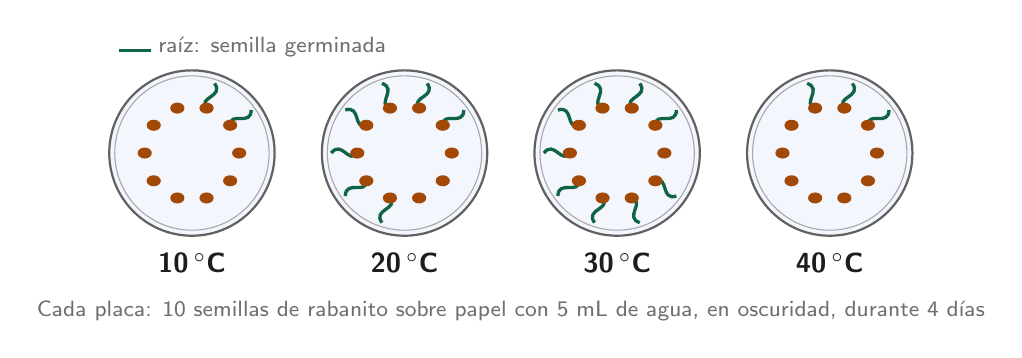
\begin{tikzpicture}[font=\small]
\foreach \i/\t/\n in {1/10/2,2/20/7,3/30/9,4/40/3}{
 \begin{scope}[shift={({2.7*(\i-1)},0)}]
  \fill[azul!6] (0,0) circle (1.05);
  \draw[tinta!70,thick] (0,0) circle (1.05);
  \draw[gris!60] (0,0) circle (0.98);
  \foreach \k in {1,...,10}{
    \pgfmathsetmacro{\ang}{36*\k}
    \ifnum\k>\n
      \fill[nar!70!black] (\ang:0.6) ellipse (0.09 and 0.07);
    \else
      \draw[menta!60!black,very thick] (\ang:0.6) .. controls ({\ang+12}:0.72) and ({\ang-12}:0.82) .. (\ang:0.93);
      \fill[nar!70!black] (\ang:0.6) ellipse (0.09 and 0.07);
    \fi}
  \node[text=tinta,font=\bfseries] at (0,-1.4) {\t\,$^\circ$C};
 \end{scope}}
\node[text=gris,font=\footnotesize] at (4.05,-2.0) {Cada placa: 10 semillas de rabanito sobre papel con 5 mL de agua, en oscuridad, durante 4 días};
\node[text=gris,font=\footnotesize,anchor=west] at (-1.05,1.35) {\textcolor{menta!60!black}{\rule{0.4cm}{1.2pt}} raíz: semilla germinada};
\end{tikzpicture}
\end{document}
